\documentclass[border=6pt]{standalone}
\usepackage{amsmath,amssymb}
\usepackage{tikz}
\usetikzlibrary{arrows.meta,calc,decorations.pathreplacing,patterns,shapes.geometric,positioning,shadings,plotmarks}

\begin{document}
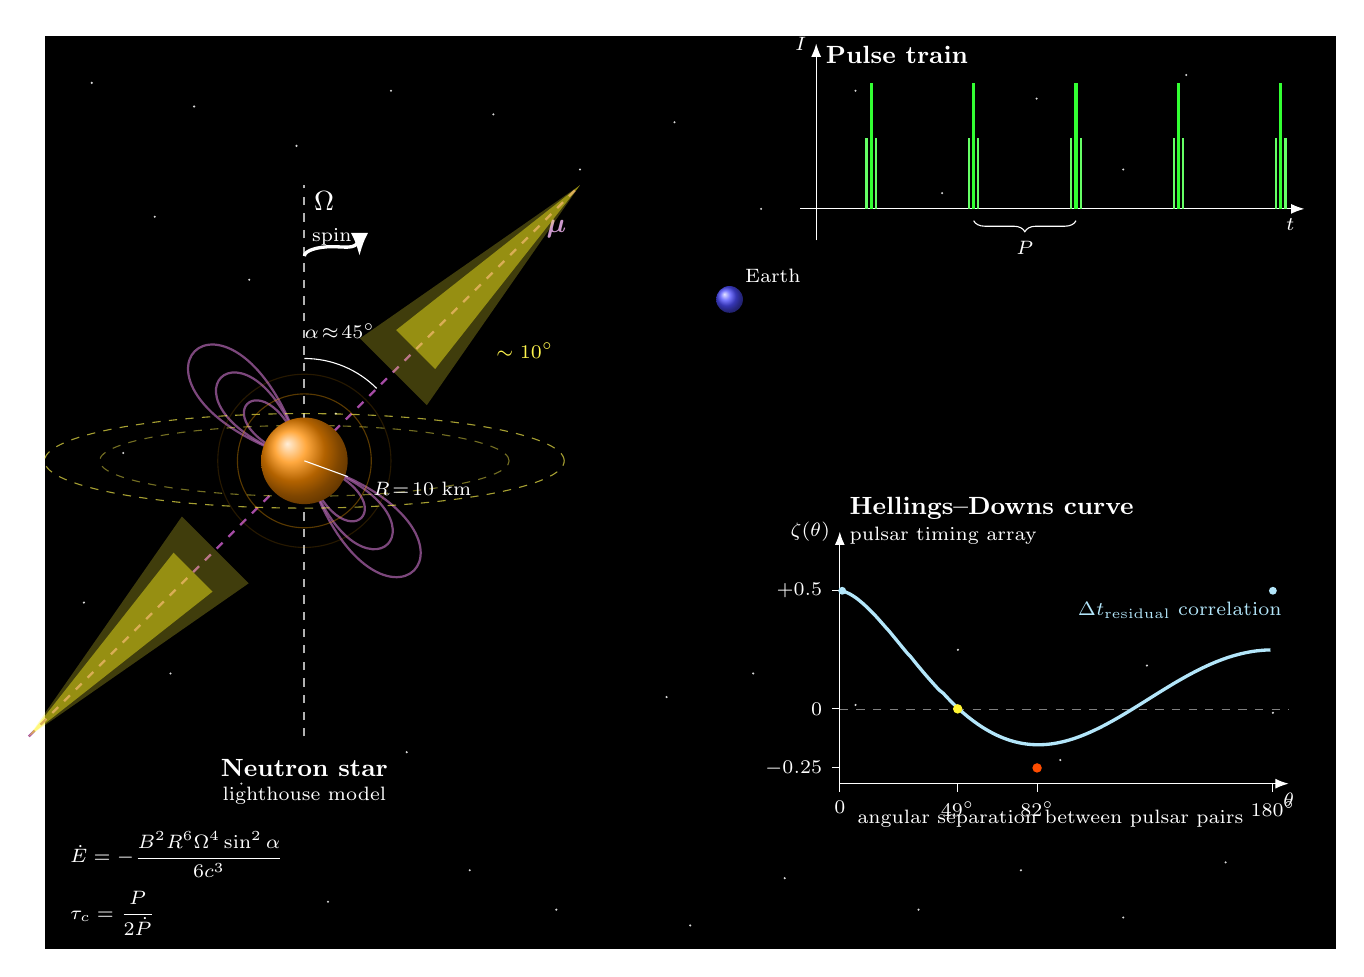
\begin{tikzpicture}[>=Latex]

  % ---- Background: deep space ----
  \fill[black] (-7.8,-6.2) rectangle (8.6,5.4);
  % scattered stars
  \foreach \x/\y in {-7.2/4.8,-6.4/3.1,-5.9/4.5,-5.2/2.3,-4.6/4.0,-4.1/0.6,-3.4/4.7,-6.8/0.1,-7.3/-1.8,-6.2/-2.7,-5.3/-4.1,-4.2/-5.6,-3.2/-3.7,-2.4/-5.2,-1.3/-5.7,0.4/-5.9,1.6/-5.3,3.3/-5.7,4.6/-5.2,5.9/-5.8,7.2/-5.1,7.8/-3.2,5.1/-3.8,6.2/-2.6,3.8/-2.4,2.5/-3.1,1.2/-2.7,0.1/-3.0,6.7/4.9,5.9/3.7,4.8/4.6,3.6/3.4,2.5/4.7,1.3/3.2,0.2/4.3,-1.0/3.7,-2.1/4.4}
    {\fill[white!85!black] (\x,\y) circle (0.015);}

  % ==================== LEFT: Neutron star lighthouse ====================
  % Rotation axis (vertical)
  \draw[white!70!black,thick,dashed] (-4.5,-3.5) -- (-4.5,3.5);
  \node[white] at (-4.25,3.3) {$\Omega$};
  \draw[->,white,very thick] (-4.5,2.6) arc (180:0:0.35 and 0.12);
  \node[white,font=\scriptsize] at (-4.15,2.85) {spin};

  % Magnetic axis (tilted about 45 deg from spin axis)
  \coordinate (NS) at (-4.5,0);
  \coordinate (Mup) at ($(NS) + (3.5,3.5)$);
  \coordinate (Mdn) at ($(NS) + (-3.5,-3.5)$);
  \draw[violet!70!white,thick,dashed] (Mdn) -- (Mup);
  \node[violet!40!white] at (-1.3,2.95) {$\boldsymbol{\mu}$};

  % Angle alpha between Omega and mu
  \draw[white,thin] (-4.5,1.3) arc (90:45:1.3);
  \node[white,font=\scriptsize] at (-4.05,1.65) {$\alpha\!\approx\!45^\circ$};

  % Magnetic field lines (purple dipolar curves, approximate loops)
  \begin{scope}[shift={(NS)},rotate=-45]
    \foreach \r in {1.3,1.9,2.5}{
      \draw[violet!60!white,thick,opacity=0.7]
        (0,0) .. controls ({\r*1.05},{\r*0.55}) and ({\r*1.05},{-\r*0.55}) .. (0,0);
      \draw[violet!60!white,thick,opacity=0.7]
        (0,0) .. controls ({-\r*1.05},{\r*0.55}) and ({-\r*1.05},{-\r*0.55}) .. (0,0);
    }
  \end{scope}

  % Upper light cone (yellow beam) along mu direction (0.707, 0.707)
  \fill[yellow!80!white,opacity=0.25]
    (Mup) -- ($(NS)+(1.6*0.707 - 0.6*0.707, 1.6*0.707 + 0.6*0.707)$) --
    ($(NS)+(1.6*0.707 + 0.6*0.707, 1.6*0.707 - 0.6*0.707)$) -- cycle;
  \fill[yellow!90!white,opacity=0.45]
    (Mup) -- ($(NS)+(2.0*0.707 - 0.35*0.707, 2.0*0.707 + 0.35*0.707)$) --
    ($(NS)+(2.0*0.707 + 0.35*0.707, 2.0*0.707 - 0.35*0.707)$) -- cycle;

  % Lower light cone
  \fill[yellow!80!white,opacity=0.25]
    (Mdn) -- ($(NS)+(-1.6*0.707 + 0.6*0.707, -1.6*0.707 - 0.6*0.707)$) --
    ($(NS)+(-1.6*0.707 - 0.6*0.707, -1.6*0.707 + 0.6*0.707)$) -- cycle;
  \fill[yellow!90!white,opacity=0.45]
    (Mdn) -- ($(NS)+(-2.0*0.707 + 0.35*0.707, -2.0*0.707 - 0.35*0.707)$) --
    ($(NS)+(-2.0*0.707 - 0.35*0.707, -2.0*0.707 + 0.35*0.707)$) -- cycle;

  % Cone half-angle label
  \node[yellow!70!white,font=\scriptsize] at (-1.7,1.4) {$\sim 10^\circ$};

  % Swept path (dashed ellipse traced by beam as star rotates)
  \draw[yellow!70!white,dashed,opacity=0.65] (-4.5,0) ellipse (3.3 and 0.6);
  \draw[yellow!70!white,dashed,opacity=0.45] (-4.5,0) ellipse (2.6 and 0.45);

  % Neutron star glowing orange body
  \shade[ball color=orange!90!yellow] (NS) circle (0.55);
  \draw[orange!70!yellow,opacity=0.35] (NS) circle (0.85);
  \draw[orange!70!yellow,opacity=0.15] (NS) circle (1.1);
  \node[white,font=\scriptsize,anchor=west] at (-3.75,-0.35) {$R\!=\!10$ km};
  \draw[white,thin] (-3.95,-0.2) -- (NS);

  % Earth symbol (small blue circle) swept by the beam
  \shade[ball color=blue!70!white] (0.9,2.05) circle (0.17);
  \node[white,font=\scriptsize] at (1.45,2.35) {Earth};

  % Label: neutron star lighthouse
  \node[white,font=\small\bfseries] at (-4.5,-3.9) {Neutron star};
  \node[white,font=\scriptsize] at (-4.5,-4.25) {lighthouse model};

  % Formula: magnetic dipole radiation
  \node[white,font=\scriptsize,anchor=west,align=left] at (-7.6,-5.0)
    {$\dot E = -\dfrac{B^{2} R^{6} \Omega^{4} \sin^{2}\alpha}{6c^{3}}$};
  \node[white,font=\scriptsize,anchor=west] at (-7.6,-5.75)
    {$\tau_{c} = \dfrac{P}{2\dot P}$};

  % ==================== TOP RIGHT: Pulse train ====================
  \draw[white,->] (1.8,3.2) -- (8.2,3.2) node[anchor=north east,font=\scriptsize] {$t$};
  \draw[white,->] (2.0,2.8) -- (2.0,5.3) node[anchor=east,font=\scriptsize] {$I$};

  % Pulse train (green spikes)
  \foreach \x in {2.7,4.0,5.3,6.6,7.9}{
    \draw[green!80!white,very thick] (\x,3.2) -- (\x,4.8);
    \draw[green!60!white,thick] (\x-0.06,3.2) -- (\x-0.06,4.1);
    \draw[green!60!white,thick] (\x+0.06,3.2) -- (\x+0.06,4.1);
  }
  % Period brackets
  \draw[white,decorate,decoration={brace,amplitude=4pt,mirror}]
    (4.0,3.05) -- (5.3,3.05);
  \node[white,font=\scriptsize] at (4.65,2.7) {$P$};

  \node[white,font=\small\bfseries,anchor=west] at (2.0,5.15) {Pulse train};

  % ==================== BOTTOM RIGHT: Hellings-Downs curve ====================
  \coordinate (HDo) at (2.3,-4.1);
  \coordinate (HDx) at (8.0,-4.1);
  \coordinate (HDy) at (2.3,-0.9);

  \draw[white,->] (HDo) -- (HDx) node[anchor=north,font=\scriptsize] {$\theta$};
  \draw[white,->] (HDo) -- (HDy) node[anchor=east,font=\scriptsize] {$\zeta(\theta)$};

  % Mapping:
  %   x = 2.3 + 5.5 * (theta/180), theta in [0, 180]
  %   y = -3.15 + 3.0 * zeta,      zeta in [-0.33, 0.5]
  % Zero baseline
  \draw[white!50!black,very thin,dashed] (2.3,-3.15) -- (8.0,-3.15);

  % x ticks
  \draw[white,thin] (2.3,-4.1) -- (2.3,-4.2);
  \node[white,font=\scriptsize,anchor=north] at (2.3,-4.2) {$0$};
  \draw[white,thin] (3.79722,-4.1) -- (3.79722,-4.2);
  \node[white,font=\scriptsize,anchor=north] at (3.79722,-4.2) {$49^\circ$};
  \draw[white,thin] (4.80556,-4.1) -- (4.80556,-4.2);
  \node[white,font=\scriptsize,anchor=north] at (4.80556,-4.2) {$82^\circ$};
  \draw[white,thin] (7.8,-4.1) -- (7.8,-4.2);
  \node[white,font=\scriptsize,anchor=north] at (7.8,-4.2) {$180^\circ$};

  % y ticks
  \draw[white,thin] (2.3,-1.65) -- (2.2,-1.65);
  \node[white,font=\scriptsize,anchor=east] at (2.2,-1.65) {$+0.5$};
  \draw[white,thin] (2.3,-3.15) -- (2.2,-3.15);
  \node[white,font=\scriptsize,anchor=east] at (2.2,-3.15) {$0$};
  \draw[white,thin] (2.3,-3.9) -- (2.2,-3.9);
  \node[white,font=\scriptsize,anchor=east] at (2.2,-3.9) {$-0.25$};

  % Hellings-Downs curve:
  %   zeta(theta) = 1.5 x ln(x) - 0.25 x + 0.5,  x = (1 - cos theta)/2
  \draw[cyan!30!white,very thick,smooth,samples=120,domain=1:179]
    plot (
      { 2.3 + 5.5*(\x)/180 },
      { -3.15 + 3.0*( 1.5*((1 - cos(\x))/2)*ln((1 - cos(\x))/2)
                      - 0.25*((1 - cos(\x))/2) + 0.5 ) }
    );

  % Endpoint markers
  \fill[cyan!30!white] (2.33056,-1.65) circle (0.05);
  \fill[cyan!30!white] (7.8,-1.65) circle (0.05);

  % Zero-crossing and minimum markers
  \fill[yellow!80!white] (3.79722,-3.15) circle (0.06);
  \fill[red!70!yellow] (4.80556,-3.9) circle (0.06);

  % Labels
  \node[white,font=\small\bfseries,anchor=west] at (2.3,-0.6)
    {Hellings--Downs curve};
  \node[white,font=\scriptsize,anchor=west] at (2.3,-0.95)
    {pulsar timing array};
  \node[cyan!30!white,font=\scriptsize,anchor=west] at (5.2,-1.9)
    {$\Delta t_{\rm residual}$ correlation};
  \node[white,font=\scriptsize,anchor=west] at (2.4,-4.55)
    {angular separation between pulsar pairs};

\end{tikzpicture}
\end{document}
